\begin{frame}{A paradox}
  \begin{mycolumns}

    \begin{column}{.5\textwidth}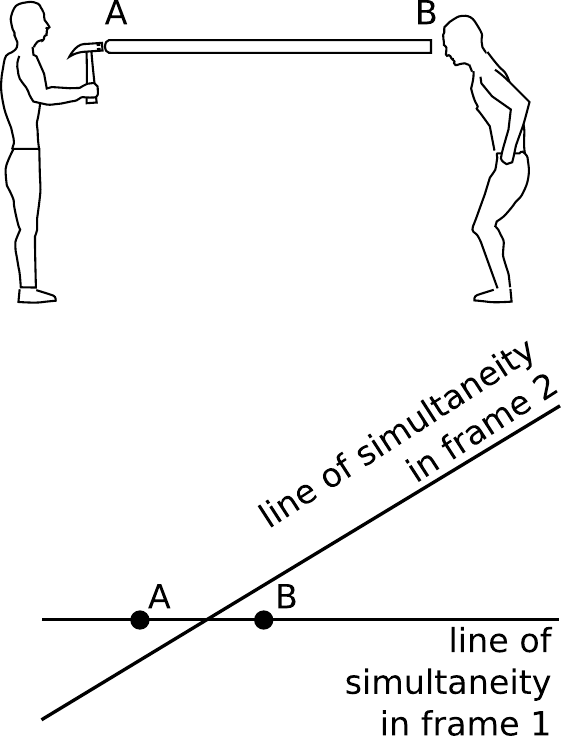
\includegraphics[width=4in]{ch02/figs/pole-paradox}\end{column}

    \begin{column}{.5\textwidth}
      \dq

      Resolve the following paradox.
      At event A, the hammer strikes one end of the rod.
      At event B, the other end moves. A and B are simultaneous in this frame of reference.
      In frame 2, B happens before A. Did the motion at the right end \emph{cause}
      the person on the left to decide to pick up the hammer and use it?

    \end{column}
  \end{mycolumns}


\end{frame}

\begin{frame}{How can they both \ldots ?}


      \dq

      Amy and Bill are flying on spaceships in opposite directions at such high velocities that
the relativistic effect on time's rate of flow is easily noticeable.
Motion is relative, so Amy considers herself to be at rest and Bill to be in motion. She says that
time is flowing normally for her, but Bill is slow. But Bill can say exactly the same thing.
How can they \emph{both} think the other is slow? Can they settle the disagreement by getting
on the radio and seeing whose voice is normal and whose sounds slowed down and Darth-Vadery?

    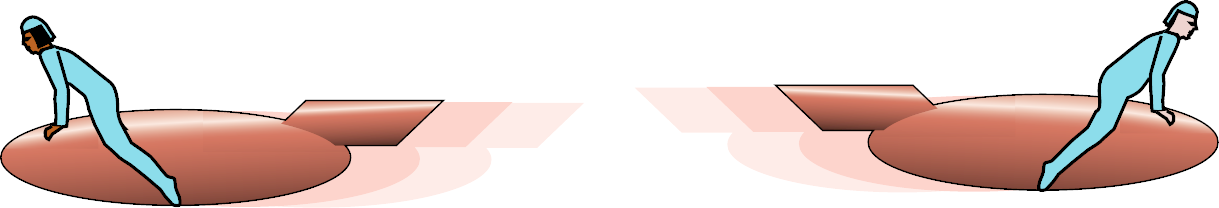
\includegraphics[width=6in]{ch02/figs/darth-vadery}


\end{frame}
